\documentclass[11pt]{article}
\usepackage[utf8]{inputenc}
\usepackage[english]{babel}
\usepackage{amsmath}
\usepackage{graphicx}
\usepackage{float}
\usepackage{lipsum}
\usepackage{multicol}
\usepackage{xcolor}
\usepackage{tabularx}
\usepackage{booktabs}
\usepackage{hyperref}
\usepackage{float}
\newcolumntype{Y}{>{\centering\arraybackslash}X}
\usepackage[left=2.00cm, right=2.00cm, top=2.00cm, bottom=2.00cm]{geometry}
\usepackage[table,xcdraw]{xcolor}
\title{AN2DL First Homework Report}

\begin{document}
    
    \begin{figure}[H]
        \raggedright
        
\includegraphics[scale=0.4]{polimi.png} \hfill 
\includegraphics[scale=0.3]{airlab.jpeg}
    \end{figure}
    
    \vspace{5mm}
    
    \begin{center}
        % Select between First and Second
        {\Large \textbf{AN2DL - First Homework Report}}\\
        \vspace{2mm}
        % Change with your Team Name
        {\Large \textbf{NeuralDropouts}}\\
        \vspace{2mm}
        % Team Members Information
        {\large Pinar Erbil,}
        {\large Sergio Pardo,}
        {\large Angela Remolina,}
        {\large Matteo Sissa}\\
        \vspace{2mm}
        % Codabench Nicknames
        {perbil,}
        {sergiopardo,}
        {angelaremolina,}
        {matteosissa}\\
        \vspace{2mm}
        % Matriculation Numbers
        {244638,}
        {243066,}
        {242814,}
        {247064}\\
        \vspace{5mm}
        \today
    \end{center}    
    \vspace{5mm}
    
    \begin{multicols}{2}
    
    \section{Introduction}
        
        Artificial intelligence has revolutionized the world we live in, the way we look at things, and the problems we aim to solve. From healthcare to transportation, AI-powered systems are enhancing efficiency, accuracy, and accessibility in ways previously unimaginable. Technologies like deep learning and deep neural networks have also allowed huge improvements in the computer vision field. 
        \\
        Medical Image Analysis falls in-between these two areas, it implements cutting edge deep learning models to boost the capability humanity has of studying our body and its composition. This is the context of the present project. It aims to \textbf{classify images of blood cells among 8 possible classes}. 

        
    \section{Problem Analysis}

       Classifying blood cells is a complex task due to the subtle differences among various cell types, which can lead to significant challenges in accurate identification.\\
        The analysis of the problem starts with the inspection of the available dataset which is composed of 13759 96x96 RGB, all labelled with an integer value ranging between 0 and 7 to representing the 8 classes of blood cells, respectively Basophil, Eosinophil, Erythroblast, Immature granulocytes, Lymphocyte, Monocyte, Neutrophil, Platelet.\\
        
        The correctness of the labels provided in the original dataset, presumably derived from expert knowledge, was assumed throughout the project.
        As for the dataset size, it was uncertain at first whether it would have been possible to rely solely on the original data without any augmentation technique. The first experimentation were therefore conducted without any augmentation to verify the system response and performance.	 

    
    \section{Method}
        \label{sec:method}
        To address the classification problem, the following methodology was employed.
        
        \subsection{Data wrangling and augmentation}
        First, the dataset was inspected using \textbf{Principal Component Analysis (PCA)}  \cite{jolliffe2016principal} to identify and remove outliers and erroneous data points.\\ 
        The cleaned dataset was split into training set (90\%), validation set (5\%) and test set (5\%) and then augmentation techniques were applied to increment the number of samples in the training set. \\
        \textbf{Augmentation} turned out to be a key step to mitigate overfitting, given the variability in imaging conditions and the limited size of the original dataset. 
        So, the augmentation step of the dataset was thoroughly redesigned, applying more advanced techniques like FourierMix \cite{fouriermix}, and CutMix \cite{cutmix}.
        Later, augmented dataset and one-hot encoded labels were fed to the model for training. 
        
        \subsection{Model design and transfer learning from pretrained model}
        Instead of training a custom model from scratch, \textbf{transfer learning} was applied.
        This approach is advantageous as it exploits the strong feature extraction capabilities of a pre-trained large model that are crucial for distinguishing subtle differences in blood cells with a limited dataset.\\
        ConvNextXLarge \cite{liu2022convnext}, trained on the ImageNet dataset \cite{deng2009imagenet}, was selected to provide the feature extraction network for the classifier of this project. It is well-suited for the goal because of its hierarchical feature extraction capabilities, able to capture fine details both at low and high level, and its robustness to image noise, very common in biomedical imaging. \cite{keras_applications} \\
        At the input side, the feature extraction network was enriched with an input layer compliant with the image size (96x96x3) and an additional augmentation layer that applies random transformations as data is fed into the system. This enhances variability in the dataset and mitigates overfitting. \\
        At the end of the ConvNextXLarge feature extraction network, there is a \textbf{custom neural network classifier} with three additional dense layers and a final output layer composed by eight output neurons corresponding to each class. The softmax function is used to normalize the output layer to a probability distribution over the classes. Dropout and batch normalization techniques are also applied in these last layers to make the model faster to train and more robust. 
        \subsection{Training, callbacks and finetuning}
        The training part was split into two parts: transfer learning and fine-tuning. In the \textbf{transfer learning} phase, the weights of the feature extraction network (ConvNextXLarge) were frozen to ensure stability and allow the training of the classifier network at the output of the model. The loss function adopted is categorical cross-entropy and back-propagation with Adaptive moment estimation (Adam) \cite{warner_optimizer} is used to update the weights. To complete the setup of the training procedure, the number of epochs was set to 15 and the batch size to 64, which seemed reasonable values as they were yielding good experimental results. 
        %todo: mention lion was a bad optimizer (experiment section)
        Callbacks such as Early-stopping and Reduce Loss Rate on Plateau were incorporated in the solution to optimize training efficiency by preventing overfitting and dynamically adjusting the learning rate when the model's performance stagnates, ensuring better convergence and improved generalization.
        The second training phase involved \textbf{fine-tuning}. The ConvNextXLarge layers were unfrozen and set as trainable to fit the specific problem. All the convolutional and depth-wise convolutional layers but the first 124 of them, were unfrozen and trained. Training procedure followed the same settings as the first training. \\    
        The final result was finally evaluated on the test set, measuring accuracy, precision, recall, f1 score and plotting a confusion matrix to examine the outcome.

        
    \section{Experiments}
		Experimentation first started from a very basic convolutional neural networks with a few layers to assess the complexity of the problem and identify the main concerns to be addressed. The initial trials only had two convolutional layers and a single dense layer at the end, and were working with unclean data. 
        Although, the local training results were promising, on CodaBench the accuracy were below 20\%.
        %TODO:  mention in conclusion or discussion section why these accuracies are so different even in the best models 
        These attempts highlighted the importance of inspecting the data in detail and increasing the amount to control overfitting. \\  
        PCA \cite{jolliffe2016principal} was therefore employed to detect outlier data points and remove them, while various augmentation techniques were devised to tailor the production of augmented data to the needs of the network. See figure \ref{fig:fig1}.

        \begin{figure}[H]
        \frame{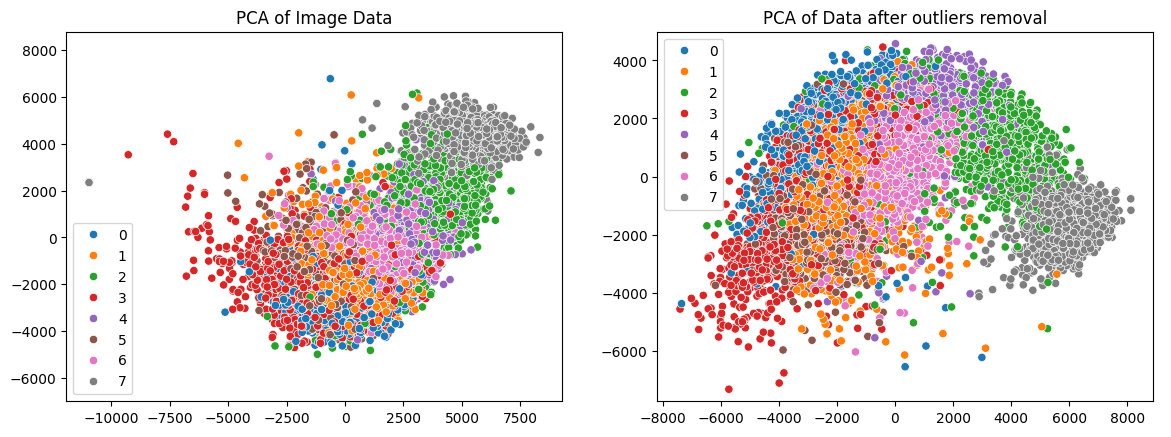
\includegraphics[width=0.6\linewidth]{images/pca.png}}
        \centering
        \caption{Plot showing PCA ditribution}
        \label{fig:fig1}
        \end{figure}

        The points located farther from the origin are identified as outliers. Upon examining these points, it becomes evident that the organizers of the competition included several irrelevant samples. Specifically, a total of 200 images of meme 1 and 1600 images of meme 2 were found, amounting to 1800  samples that were deleted from the dataset. See figure \ref{fig:fig2}

        \begin{figure}[H]
        \frame{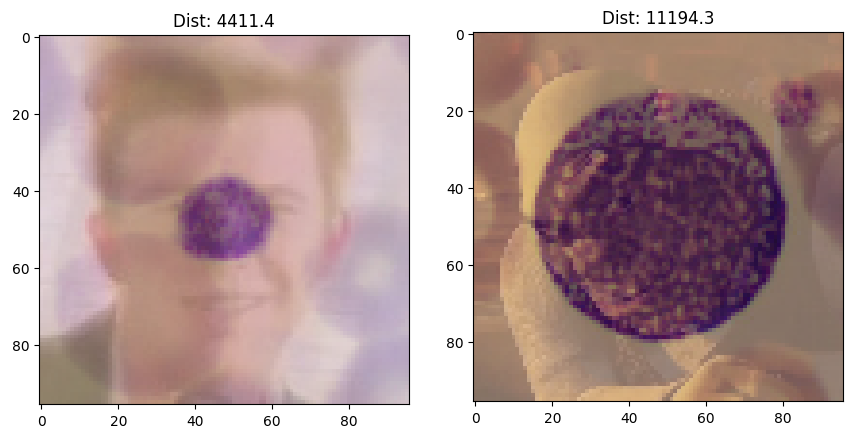
\includegraphics[width=0.7\linewidth]{images/memes.png}}
        \centering
        \caption{Memes found in dataset}
        \label{fig:fig2}
        \end{figure}

        After establishing a clean data set, transfer learning was implemented using VGG \cite{simonyan2014very}, ConvNextBase \cite{liu2022convnet}, ConvNextXLarge\cite{liu2022convnet} as possible model options. 
        They were all used as feature extraction networks, completing them with an input layer suitable for the input images of the problem and a classification network at the end composed of three dense fully-connected layers. \\
        Several different settings were employed while using these models. Initially, simple models with no augmentation were implemented. Then, fine-tuning and augmentation were utilized in the pipeline for the more complex models. All the results are presented in Table \ref{tab:Performance} with their corresponding settings. \\
         
        From these results it can be concluded that using transfer learning leads to better performances. Although ConvNext models outperformed VGG, there is no clear winner between the ConvNext models.
        It was also proven that by carefully balancing class weights and fine-tuning key hyperparameters (such as the number of epochs, batch size, patience, ...) it is possible to achieve the same accuracy (85\%) with a ConvNext-Base model as with a ConvNext-Large model. Given that ConvNext-Base is significantly lighter and more computationally efficient, it presents a compelling alternative to ConvNext-Large, offering equivalent performance while requiring fewer resources. This underscores the effectiveness of optimization techniques in maximizing the efficiency of machine learning models.
        
        \color{red} MORE DISCUSSION HERE AFTER XLARGE COMES and block train comes \color{black} 
        
        \begin{table*}[t]
 \hskip-1.5cm
\begin{tabular}{lccc|cccc|c|}
\cline{5-9}
                                                                                     & \multicolumn{1}{l}{}                                       & \multicolumn{1}{l}{}                                               & \multicolumn{1}{l|}{} & \multicolumn{4}{c|}{\cellcolor[HTML]{C0C0C0}Local Results}                                                                                                                                                      & \multicolumn{1}{l|}{\cellcolor[HTML]{C0C0C0}CodaBench} \\ \hline
\rowcolor[HTML]{C0C0C0} 
\multicolumn{1}{|l|}{\cellcolor[HTML]{C0C0C0}\textbf{Model}}                         & \multicolumn{1}{c|}{\cellcolor[HTML]{C0C0C0}\textbf{Data}} & \multicolumn{1}{c|}{\cellcolor[HTML]{C0C0C0}\textbf{Augmentation}} & \textbf{Fine-tuning}  & \multicolumn{1}{c|}{\cellcolor[HTML]{C0C0C0}\textbf{Accuracy}} & \multicolumn{1}{c|}{\cellcolor[HTML]{C0C0C0}\textbf{Precision}} & \multicolumn{1}{c|}{\cellcolor[HTML]{C0C0C0}\textbf{Recall}} & \textbf{F1}   & \textbf{Accuracy}                                      \\ \hline
\multicolumn{1}{|l|}{Base Model}                                                     & \multicolumn{1}{c|}{Unclean}                               & \multicolumn{1}{c|}{No}                                            & No                    & \multicolumn{1}{c|}{0.7}                                       & \multicolumn{1}{c|}{0.72}                                       & \multicolumn{1}{c|}{0.7}                                     & 0.68          & 0.14                                                   \\ \hline
\multicolumn{1}{|l|}{VGG}                                                            & \multicolumn{1}{c|}{Clean}                                 & \multicolumn{1}{c|}{No}                                            & Yes                   & \multicolumn{1}{c|}{0.87}                                      & \multicolumn{1}{c|}{0.91}                                       & \multicolumn{1}{c|}{0.87}                                    & 0.88          & 0.49                                                   \\ \hline
\multicolumn{1}{|l|}{ConvNextBase}                                                   & \multicolumn{1}{c|}{Clean}                                 & \multicolumn{1}{c|}{Yes}                                           & Yes                   & \multicolumn{1}{c|}{0.97}                                      & \multicolumn{1}{c|}{0.97}                                       & \multicolumn{1}{c|}{0.97}                                    & 0.97          & \textbf{0.85}                                          \\ \hline
\multicolumn{1}{|l|}{ConvNextLarge}                                                  & \multicolumn{1}{c|}{Clean}                                 & \multicolumn{1}{c|}{Yes}                                           & Yes                   & \multicolumn{1}{c|}{\textbf{0.98}}                             & \multicolumn{1}{c|}{\textbf{0.98}}                              & \multicolumn{1}{c|}{\textbf{0.98}}                           & \textbf{0.98} & \textbf{0.85}                                          \\ \hline
\multicolumn{1}{|l|}{ConvNextXLarge}                                                 & \multicolumn{1}{c|}{Clean}                                 & \multicolumn{1}{c|}{No}                                            & No                    & \multicolumn{1}{c|}{0.95}                                      & \multicolumn{1}{c|}{0.95}                                       & \multicolumn{1}{c|}{0.95}                                    & 0.95          & 0.74                                                   \\ \hline
\multicolumn{1}{|l|}{ConvNextXLarge}                                                 & \multicolumn{1}{c|}{Clean}                                 & \multicolumn{1}{c|}{Yes}                                           & Yes                   & \multicolumn{1}{c|}{}                                          & \multicolumn{1}{c|}{}                                           & \multicolumn{1}{c|}{}                                        &               &                                                        \\ \hline
\multicolumn{1}{|l|}{\begin{tabular}[c]{@{}l@{}}Block\\ ConvNextXlarge\end{tabular}} & \multicolumn{1}{c|}{Clean}                                 & \multicolumn{1}{c|}{Yes}                                           & Yes                   & \multicolumn{1}{c|}{}                                          & \multicolumn{1}{c|}{}                                           & \multicolumn{1}{c|}{}                                        &               &                                                        \\ \hline
\end{tabular}
        \caption{Summary of the models' performances}
        \label{tab:Performance}
\end{table*}
        


        
    \section{Results}
		The final model presented in this paper achieved an overall \textbf{accuracy of 85\%} on test data. Compared to the initial attempts that were made with very simple models, this shows an improvement of \textbf{around 70 percentage points} throughout the design process for this solution. The two most important contributions to this achievement can be attributed to using \textbf{augmentation} and \textbf{transfer learning} techniques to craft a precise solution for the problem at hand.

        \color{red}add image of confusion matrix of the best model \color{black} 
        
    \section{Discussion}
        The final achievement shows a robust solution to distinguish blood cells even in the case of classes with very low variability and subtle differences. At the same time, the reliance on pre-trained weights from ImageNet, a non-biomedical dataset, could limit the model's ability to capture domain-specific features, particularly those unique to blood cell microscopy images. 

        
    \section{Conclusions}
	In this work, we proposed a robust solution for blood cell classification leveraging transfer learning with the ConvNeXt-XLarge backbone and advanced data augmentation techniques. The approach effectively addressed challenges, achieving competitive performance across most cell types. \\
    Future work could focus on generating synthetic data for rare classes or collecting additional images for easier and more precise training. It is also possible to experiment with lighter models for transfer learning and verify the change in performance.
\cite{mixup}
        


        \bibliography{references}
        \bibliographystyle{abbrv}
    
    
    \end{multicols}
\end{document}